% Source PDF page 385 (printed p. 371)
\begin{figure}[htbp]\centering
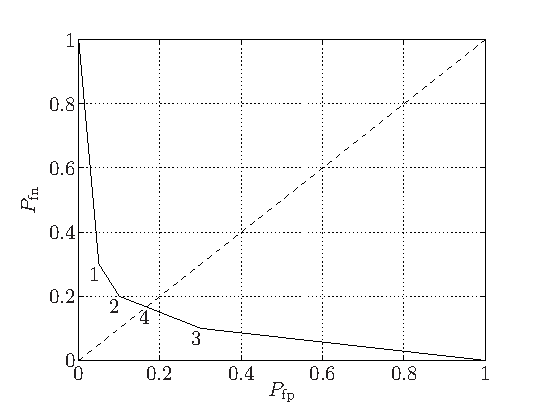
\includegraphics[width=.72\textwidth]{figures/ch07-figure-4.pdf}
\caption*{图7.4\quad 对（7.15）中的矩阵 $P$，假阴性概率与假阳性概率的最优权衡曲线。标为1至3的顶点对应确定性检测器；标为4的点对应随机化的极小极大检测器。虚线为 $P_{\mathrm{fn}}=P_{\mathrm{fp}}$，即两种错误概率相等的点。}
\end{figure}
上式是观测到 $X=k$ 时的判决。这称为\emph{似然比门限检验}：如果比值 $p_k/q_k$ 超过门限 $W_{12}/W_{21}$，检验为阴性，即 $\widehat\theta=1$；否则为阳性。选择不同门限，会得到假阳性与假阴性错误概率不同的确定性Pareto最优检测器。该结果称为\emph{Neyman--Pearson引理}。

似然比检测器并未给出全部Pareto最优检测器；它们是分段线性最优权衡曲线上的顶点。

\begin{origexample}{7.4}
考虑 $n=4$ 的二元假设检验例子，
\begin{equation}
 P=\begin{bmatrix}
 0.70&0.10\\0.20&0.10\\0.05&0.70\\0.05&0.10
 \end{bmatrix}.\tag{7.15}
\end{equation}
$P_{\mathrm{fn}}$ 与 $P_{\mathrm{fp}}$ 的最优权衡曲线，即接收者工作特征曲线，见图7.4。左端点对应始终输出阴性、与 $X$ 观测值无关的检测器；右端点对应始终输出阳性的检测器。标为1、2、3的顶点，分别对应确定性检测器
\[
 T^{(1)}=\begin{bmatrix}1&1&0&1\\0&0&1&0\end{bmatrix},\qquad
 T^{(2)}=\begin{bmatrix}1&1&0&0\\0&0&1&1\end{bmatrix},
\]

% Source PDF page 386 (printed p. 372)
\[
 T^{(3)}=\begin{bmatrix}1&0&0&0\\0&1&1&1\end{bmatrix}.
\]
标为4的点对应非确定性检测器
\[
 T^{(4)}=\begin{bmatrix}1&2/3&0&0\\0&1/3&1&1\end{bmatrix},
\]
它是极小极大检测器，假阳性与假阴性的概率相等，本例中均为 $1/6$。每个确定性检测器至少有一种错误概率超过 $1/6$，因此这是随机化检测器优于所有确定性检测器的例子。
\end{origexample}

\subsection{稳健检测器}
到目前为止，假设给出每个参数 $\theta$ 下观测变量 $X$ 分布的矩阵 $P$ 已知。本节考虑这些分布未知、但给定某些先验信息的情形。设 $P\in\mathcal P$，其中 $\mathcal P$ 为可能分布的集合。对由 $T$ 刻画的随机化检测器，检测概率矩阵 $D$ 现在依赖于具体的 $P$。我们按 $P\in\mathcal P$ 中的最坏值评价错误概率。定义\emph{最坏情形检测概率矩阵} $D^{\mathrm{wc}}$ 为
\[
 D_{ij}^{\mathrm{wc}}=\sup_{P\in\mathcal P}D_{ij},\qquad
 i,j=1,\ldots,m,\quad i\ne j,
\]
以及
\[
 D_{ii}^{\mathrm{wc}}=\inf_{P\in\mathcal P}D_{ii},\qquad i=1,\ldots,m.
\]
非对角元给出 $P\in\mathcal P$ 中最大可能的错误概率，对角元给出最小可能的检测概率。注意，一般有 $\sum_{i=1}^nD_{ij}^{\mathrm{wc}}\ne1$，即最坏情形检测概率矩阵的各列和不一定等于一。

定义最坏情形错误概率为
\[
 P_i^{\mathrm{wce}}=1-D_{ii}^{\mathrm{wc}}.
\]
因此，$P_i^{\mathrm{wce}}$ 是 $\theta=i$ 时，在 $\mathcal P$ 所有可能分布中的最大错误概率。

用最坏情形检测概率矩阵，或最坏情形错误概率向量，可以构造多种稳健检测器设计问题。本节其余部分集中讨论稳健极小极大检测器，以此为代表说明这些思想。

定义\emph{稳健极小极大检测器}，使所有假设下的最坏错误概率最小，即最小化
\[
 \max_iP_i^{\mathrm{wce}}
 =\max_{i=1,\ldots,m}\sup_{P\in\mathcal P}(1-(TP)_{ii})
 =1-\min_{i=1,\ldots,m}\inf_{P\in\mathcal P}(TP)_{ii}.
\]
稳健极小极大检测器最小化所有 $m$ 个假设、所有 $P\in\mathcal P$ 中最坏的错误概率。

% Source PDF page 387 (printed p. 373)
\subsubsection*{有限 $\mathcal P$ 的稳健极小极大检测器}
可能分布集合有限时，稳健极小极大检测器设计很容易写成线性规划。设 $\mathcal P=\{P_1,\ldots,P_k\}$，可求解
\[
\begin{array}{ll}
\text{最大化}&\displaystyle\min_{i=1,\ldots,m}\inf_{P\in\mathcal P}(TP)_{ii}
 =\min_{i=1,\ldots,m}\min_{j=1,\ldots,k}(TP_j)_{ii}\\
\text{满足}&t_i\succeq0,\quad\one^{\T}t_i=1,\quad i=1,\ldots,n
\end{array}
\]
得到稳健极小极大检测器。目标为分段线性凹函数，因此问题可表示为线性规划。也可以将可能分布集取为多面体 $\conv\mathcal P$，相应最坏情形检测矩阵和稳健极小极大检测器都不变。

\subsubsection*{多面体 $\mathcal P$ 的稳健极小极大检测器}
当 $\mathcal P$ 是由线性等式与不等式描述的多面体时，也能高效地将稳健极小极大检测器问题写成线性规划。这一形式较不直观，要依靠 $\mathcal P$ 的对偶表示。

为简化讨论，假设 $\mathcal P$ 具有形式
\begin{equation}
 \mathcal P=\left\{P=\begin{bmatrix}p_1&\cdots&p_m\end{bmatrix}
 \ \middle|\ A_kp_k=b_k,\ \one^{\T}p_k=1,\ p_k\succeq0\right\}.\tag{7.16}
\end{equation}
换言之，对每个分布 $p_k$，给定某些期望值 $A_kp_k=b_k$，它们可以是已知的矩、概率等。推广到给定期望不等式的情形很直接。

稳健极小极大设计问题为
\[
\begin{array}{ll}
\text{最大化}&\gamma\\
\text{满足}&\inf\{\widetilde t_i^{\T}p\mid A_ip=b_i,\ \one^{\T}p=1,\ p\succeq0\}\ge\gamma,
 \quad i=1,\ldots,m,\\
&t_i\succeq0,\quad\one^{\T}t_i=1,\quad i=1,\ldots,n,
\end{array}
\]
其中 $\widetilde t_i^{\T}$ 表示 $T$ 的第 $i$ 行，因此 $(TP)_{ii}=\widetilde t_i^{\T}p_i$。由线性规划对偶性，
\[
\begin{aligned}
 &\inf\{\widetilde t_i^{\T}p\mid A_ip=b_i,\ \one^{\T}p=1,\ p\succeq0\}\\
 &\qquad=\sup\{\nu^{\T}b_i+\mu\mid A_i^{\T}\nu+\mu\one\preceq\widetilde t_i\}.
\end{aligned}
\]
据此，稳健极小极大检测器设计可表示为线性规划
\[
\begin{array}{ll}
\text{最大化}&\gamma\\
\text{满足}&\nu_i^{\T}b_i+\mu_i\ge\gamma,\quad i=1,\ldots,m,\\
&A_i^{\T}\nu_i+\mu_i\one\preceq\widetilde t_i,\quad i=1,\ldots,m,\\
&t_i\succeq0,\quad\one^{\T}t_i=1,\quad i=1,\ldots,n,
\end{array}
\]
变量为 $\nu_1,\ldots,\nu_m$、$\mu_1,\ldots,\mu_n$ 及 $T$，后者的列为 $t_i$，行为 $\widetilde t_i^{\T}$。

\begin{origexample}{7.5}
\textbf{稳健二元假设检验。}设 $m=2$，且（7.16）中的 $\mathcal P$ 由下列数据定义：
\[
 A_1=A_2=A=\begin{bmatrix}a_1&a_2&\cdots&a_n\\
 a_1^2&a_2^2&\cdots&a_n^2\end{bmatrix},\qquad
 b_1=\begin{bmatrix}\alpha_1\\\alpha_2\end{bmatrix},\qquad
 b_2=\begin{bmatrix}\beta_1\\\beta_2\end{bmatrix}.
\]
对这个 $\mathcal P$ 设计稳健极小极大检测器，可以解释为二元假设检验问题：根据随机变量 $X\in\{a_1,\ldots,a_n\}$ 的一次观测，在以下两个假设中选择：

% Source PDF page 388 (printed p. 374)
\begin{enumerate}
\item $\E X=\alpha_1$、$\E X^2=\alpha_2$；
\item $\E X=\beta_1$、$\E X^2=\beta_2$。
\end{enumerate}
令 $\widetilde t^{\T}$ 为 $T$ 的第一行，则 $(\one-\widetilde t)^{\T}$ 为第二行。给定 $\widetilde t$，最坏情形的正确检测概率为
\[
\begin{aligned}
 D_{11}^{\mathrm{wc}}
 &=\inf\left\{\widetilde t^{\T}p\ \middle|\
 \sum_{i=1}^na_ip_i=\alpha_1,\ \sum_{i=1}^na_i^2p_i=\alpha_2,
 \ \one^{\T}p=1,\ p\succeq0\right\},\\
 D_{22}^{\mathrm{wc}}
 &=\inf\left\{(\one-\widetilde t)^{\T}p\ \middle|\
 \sum_{i=1}^na_ip_i=\beta_1,\ \sum_{i=1}^na_i^2p_i=\beta_2,
 \ \one^{\T}p=1,\ p\succeq0\right\}.
\end{aligned}
\]
利用线性规划对偶性，$D_{11}^{\mathrm{wc}}$ 可表示为线性规划
\[
\begin{array}{ll}
\text{最大化}&z_0+z_1\alpha_1+z_2\alpha_2\\
\text{满足}&z_0+a_iz_1+a_i^2z_2\le\widetilde t_i,\quad i=1,\ldots,n
\end{array}
\]
的最优值，变量为 $z_0,z_1,z_2\in\R$。类似地，$D_{22}^{\mathrm{wc}}$ 是线性规划
\[
\begin{array}{ll}
\text{最大化}&w_0+w_1\beta_1+w_2\beta_2\\
\text{满足}&w_0+a_iw_1+a_i^2w_2\le1-\widetilde t_i,\quad i=1,\ldots,n
\end{array}
\]
的最优值，变量为 $w_0,w_1,w_2\in\R$。为得到极小极大检测器，要最大化 $D_{11}^{\mathrm{wc}}$ 与 $D_{22}^{\mathrm{wc}}$ 的最小值，即求解
\[
\begin{array}{ll}
\text{最大化}&\gamma\\
\text{满足}&z_0+z_1\alpha_2+z_2\alpha_2\ge\gamma,\\
&w_0+\beta_1w_1+\beta_2w_2\ge\gamma,\\
&z_0+z_1a_i+z_2a_i^2\le\widetilde t_i,\quad i=1,\ldots,n,\\
&w_0+w_1a_i+w_2a_i^2\le1-\widetilde t_i,\quad i=1,\ldots,n,\\
&0\preceq\widetilde t\preceq\one.
\end{array}
\]
变量为 $z_0,z_1,z_2,w_0,w_1,w_2$ 和 $\widetilde t$。
\end{origexample}

\section{Chebyshev界与Chernoff界}
本节考虑两类经典的集合概率界，并说明它们的推广形式都能写成凸优化问题。原来的经典界对应具有解析解的简单凸优化问题；更一般情形的凸优化形式，可以计算更好的界，或者处理更复杂的情形。

\subsection{Chebyshev界}
Chebyshev界根据某些函数的已知期望，例如均值与方差，给出某个集合的概率上界。最简单的例子是Markov不等式：若 $X$ 是 $\R_+$ 上的随机变量，$\E X=\mu$，则无论 $X$ 的分布如何，都有 $\Prob(X\ge1)\le\mu$。

% Source PDF page 389 (printed p. 375)
另一个简单例子是Chebyshev界：若 $X$ 是 $\R$ 上的随机变量，$\E X=\mu$，$\E(X-\mu)^2=\sigma^2$，则无论分布如何，都有 $\Prob(\abs{X-\mu}\ge1)\le\sigma^2$。这些简单界背后的思想，可以推广为用凸优化计算概率界。

设 $X$ 是 $S\subseteq\R^m$ 上的随机变量，$C\subseteq S$ 是我们希望对其概率 $\Prob(X\in C)$ 求界的集合。用 $\one_C$ 表示 $C$ 的0--1指示函数，即 $z\in C$ 时 $\one_C(z)=1$，$z\notin C$ 时 $\one_C(z)=0$。

关于分布的先验知识，是一些函数的已知期望：
\[
 \E f_i(X)=a_i,\qquad i=1,\ldots,n,
\]
其中 $f_i:\R^m\to\R$。令 $f_0$ 为值恒等于一的常函数，总有 $\E f_0(X)=a_0=1$。考虑这些函数的线性组合
\[
 f(z)=\sum_{i=0}^nx_if_i(z),
\]
其中 $x_i\in\R$，$i=0,\ldots,n$。由已知的 $\E f_i(X)$，可得 $\E f(X)=a^{\T}x$。

假设 $f$ 满足对所有 $z\in S$ 有 $f(z)\ge\one_C(z)$，即在 $S$ 上逐点不小于 $C$ 的指示函数，则
\[
 \E f(X)=a^{\T}x\ge\E\one_C(X)=\Prob(X\in C).
\]
换言之，$a^{\T}x$ 是 $\Prob(X\in C)$ 的上界，对所有支撑于 $S$、满足 $\E f_i(X)=a_i$ 的分布都有效。

通过求解
\begin{equation}
\begin{array}{ll}
\text{最小化}&x_0+a_1x_1+\cdots+a_nx_n\\
\text{满足}&f(z)=\sum_{i=0}^nx_if_i(z)\ge1,\quad z\in C,\\
&f(z)=\sum_{i=0}^nx_if_i(z)\ge0,\quad z\in S,\ z\notin C,
\end{array}\tag{7.17}
\end{equation}
可寻找这类上界中最好的一个，变量为 $x\in\R^{n+1}$。该问题总凸，因为约束可表示为
\[
 g_1(x)=1-\inf_{z\in C}f(z)\le0,\qquad
 g_2(x)=-\inf_{z\in S\setminus C}f(z)\le0,
\]
其中 $g_1,g_2$ 凸。问题（7.17）也可视为\emph{半无限线性规划}：目标线性，包含无穷多个线性不等式，每个 $z\in S$ 对应一个。

简单情形下，（7.17）可解析求解。例如，取 $S=\R_+$、$C=[1,\infty)$、$f_0(z)=1$、$f_1(z)=z$，先验信息为 $\E f_1(X)=\E X=\mu\le1$。条件 $f(z)\ge0$ 对所有 $z\in S$ 成立，化为 $x_0\ge0$、$x_1\ge0$。条件 $f(z)\ge1$ 对所有 $z\in C$ 成立，即 $x_0+x_1z\ge1$ 对所有 $z\ge1$ 成立，化为 $x_0+x_1\ge1$。因此（7.17）成为
\[
\begin{array}{ll}
\text{最小化}&x_0+\mu x_1\\
\text{满足}&x_0\ge0,\quad x_1\ge0,\\
&x_0+x_1\ge1.
\end{array}
\]

% Source PDF page 390 (printed p. 376)
由于 $0\le\mu\le1$，这个简单线性规划的最优点为 $x_0=0$、$x_1=1$，得到经典Markov界 $\Prob(X\ge1)\le\mu$。其他情况下，可以用凸优化求解（7.17）。

\begin{quote}\textbf{说明7.1\quad 对偶性与Chebyshev界问题。}
Chebyshev界问题（7.17）给出对所有满足指定期望约束的概率测度都成立的 $\Prob(X\in C)$ 上界。因此，可将（7.17）看作对以下无限维问题的最优值求界：
\begin{equation}
\begin{array}{ll}
\text{最大化}&\displaystyle\int_C\pi(\mathrm dz)\\
\text{满足}&\displaystyle\int_S f_i(z)\pi(\mathrm dz)=a_i,\quad i=1,\ldots,n,\\
&\displaystyle\int_S\pi(\mathrm dz)=1,\\
&\pi\ge0,
\end{array}\tag{7.18}
\end{equation}
变量为测度 $\pi$，$\pi\ge0$ 表示它是非负测度。

Chebyshev问题（7.17）为（7.18）求界，因此两者由对偶性联系起来并不意外。虽然半无限与无限维问题超出本书范围，我们仍可形式地构造（7.17）的对偶：引入拉格朗日乘子函数 $p:S\to\R$，其中 $p(z)$ 是不等式 $f(z)\ge1$（$z\in C$）或 $f(z)\ge0$（$z\in S\setminus C$）的乘子。将有限维中的求和改为对 $z$ 积分，得到形式对偶
\[
\begin{array}{ll}
\text{最大化}&\displaystyle\int_Cp(z)\,\mathrm dz\\
\text{满足}&\displaystyle\int_Sf_i(z)p(z)\,\mathrm dz=a_i,\quad i=1,\ldots,n,\\
&\displaystyle\int_Sp(z)\,\mathrm dz=1,\\
&p(z)\ge0,\quad\text{对所有 }z\in S,
\end{array}
\]
优化变量为函数 $p$。这与（7.18）本质上相同。
\end{quote}

\subsubsection*{已知一阶与二阶矩时的概率界}
例如，设 $S=\R^m$，给定随机变量 $X$ 的一阶与二阶矩：
\[
 \E X=a\in\R^m,\qquad\E XX^{\T}=\Sigma\in\mathbf S^m.
\]
也就是说，已知 $m$ 个函数 $z_i$（$i=1,\ldots,m$）以及 $m(m+1)/2$ 个函数 $z_iz_j$（$i,j=1,\ldots,m$）的期望，但没有分布的其他信息。

这时可将 $f$ 写成一般二次函数
\[
 f(z)=z^{\T}Pz+2q^{\T}z+r,
\]
变量，也就是前面讨论中的向量 $x$，为 $P\in\mathbf S^m$、$q\in\R^m$、$r\in\R$。利用已知的一阶与二阶矩，有
\[
\begin{aligned}
 \E f(X)&=\E(X^{\T}PX+2q^{\T}X+r)\\
 &=\E\tr(PXX^{\T})+2\E q^{\T}X+r\\
 &=\tr(\Sigma P)+2q^{\T}a+r.
\end{aligned}
\]

% Source PDF page 391 (printed p. 377)
$f(z)\ge0$ 对所有 $z$ 成立，可表示为线性矩阵不等式
\[
 \begin{bmatrix}P&q\\q^{\T}&r\end{bmatrix}\succeq0.
\]
特别地，$P\succeq0$。

现设 $C$ 是一个开多面体的补集，
\[
 C=\R^m\setminus\mathcal P,\qquad
 \mathcal P=\{z\mid a_i^{\T}z<b_i,\ i=1,\ldots,k\}.
\]
对所有 $z\in C$ 要求 $f(z)\ge1$，等价于对 $i=1,\ldots,k$ 要求
\[
 a_i^{\T}z\ge b_i\quad\Longrightarrow\quad z^{\T}Pz+2q^{\T}z+r\ge1.
\]
这又可表示为：存在 $\tau_1,\ldots,\tau_k\ge0$，使
\[
 \begin{bmatrix}P&q\\q^{\T}&r-1\end{bmatrix}
 \succeq\tau_i\begin{bmatrix}0&a_i/2\\a_i^{\T}/2&-b_i\end{bmatrix},
 \qquad i=1,\ldots,k,
\]
见第B.2节。

综合可得，Chebyshev界问题（7.17）可写为
\begin{equation}
\begin{array}{ll}
\text{最小化}&\tr(\Sigma P)+2q^{\T}a+r\\
\text{满足}&\displaystyle\begin{bmatrix}P&q\\q^{\T}&r-1\end{bmatrix}
 \succeq\tau_i\begin{bmatrix}0&a_i/2\\a_i^{\T}/2&-b_i\end{bmatrix},
 \quad i=1,\ldots,k,\\[3pt]
&\tau_i\ge0,\quad i=1,\ldots,k,\\[3pt]
&\displaystyle\begin{bmatrix}P&q\\q^{\T}&r\end{bmatrix}\succeq0.
\end{array}\tag{7.19}
\end{equation}
这是关于 $P,q,r,\tau_1,\ldots,\tau_k$ 的半正定规划。设最优值为 $\alpha$，它就是所有均值为 $a$、二阶矩为 $\Sigma$ 的分布下 $\Prob(X\in C)$ 的上界。反过来，$1-\alpha$ 是 $\Prob(X\in\mathcal P)$ 的下界。

\begin{quote}\textbf{说明7.2\quad 对偶性与Chebyshev界问题。}
与（7.19）对应的对偶半正定规划可写为
\[
\begin{array}{ll}
\text{最大化}&\sum_{i=1}^k\lambda_i\\
\text{满足}&a_i^{\T}z_i\ge b\lambda_i,\quad i=1,\ldots,k,\\[3pt]
&\displaystyle\sum_{i=1}^k\begin{bmatrix}Z_i&z_i\\z_i^{\T}&\lambda_i\end{bmatrix}
 \preceq\begin{bmatrix}\Sigma&a\\a^{\T}&1\end{bmatrix},\\[3pt]
&\displaystyle\begin{bmatrix}Z_i&z_i\\z_i^{\T}&\lambda_i\end{bmatrix}\succeq0,
 \quad i=1,\ldots,k.
\end{array}
\]
变量为 $Z_i\in\mathbf S^m$、$z_i\in\R^m$、$\lambda_i\in\R$，$i=1,\ldots,k$。由于（7.19）严格可行，强对偶成立，且对偶最优值可取到。

这个对偶问题有一个有趣的概率解释。设 $Z_i,z_i,\lambda_i$ 对偶可行，且 $\lambda$ 的前 $r$ 个分量为正，其余为零。

% Source PDF page 392 (printed p. 378)
为简单起见，还假设 $\sum_{i=1}^k\lambda_i<1$。定义
\[
\begin{aligned}
 x_i&=(1/\lambda_i)z_i,\quad i=1,\ldots,r,\\
 w_0&=\frac1\mu\left(a-\sum_{i=1}^r\lambda_ix_i\right),\\
 W&=\frac1\mu\left(\Sigma-\sum_{i=1}^r\lambda_ix_ix_i^{\T}\right),
\end{aligned}
\]
其中 $\mu=1-\sum_{i=1}^k\lambda_i$。用这些定义，对偶可行性约束可写为
\[
 a_i^{\T}x_i\ge b_i,\qquad i=1,\ldots,r,
\]
以及
\[
 \sum_{i=1}^r\lambda_i\begin{bmatrix}x_ix_i^{\T}&x_i\\x_i^{\T}&1\end{bmatrix}
 +\mu\begin{bmatrix}W&w_0\\w_0^{\T}&1\end{bmatrix}
 =\begin{bmatrix}\Sigma&a\\a^{\T}&1\end{bmatrix}.
\]
此外，由对偶可行性，
\[
\begin{aligned}
 \mu\begin{bmatrix}W&w_0\\w_0^{\T}&1\end{bmatrix}
 &=\begin{bmatrix}\Sigma&a\\a^{\T}&1\end{bmatrix}
   -\sum_{i=1}^r\lambda_i\begin{bmatrix}x_ix_i^{\T}&x_i\\x_i^{\T}&1\end{bmatrix}\\
 &=\begin{bmatrix}\Sigma&a\\a^{\T}&1\end{bmatrix}
   -\sum_{i=1}^r\begin{bmatrix}(1/\lambda_i)z_iz_i^{\T}&z_i\\z_i^{\T}&\lambda_i\end{bmatrix}\\
 &\succeq\begin{bmatrix}\Sigma&a\\a^{\T}&1\end{bmatrix}
   -\sum_{i=1}^r\begin{bmatrix}Z_i&z_i\\z_i^{\T}&\lambda_i\end{bmatrix}\\
 &\succeq0.
\end{aligned}
\]
因此，$W\succeq w_0w_0^{\T}$，可分解为 $W-w_0w_0^{\T}=\sum_{i=1}^sw_iw_i^{\T}$。考虑具有以下分布的离散随机变量 $X$。如果 $s\ge1$，取
\[
\begin{array}{lll}
 X=x_i&\text{概率为 }\lambda_i,&i=1,\ldots,r,\\
 X=w_0+\sqrt{s}\,w_i&\text{概率为 }\mu/(2s),&i=1,\ldots,s,\\
 X=w_0-\sqrt{s}\,w_i&\text{概率为 }\mu/(2s),&i=1,\ldots,s.
\end{array}
\]
如果 $s=0$，取
\[
\begin{array}{lll}
 X=x_i&\text{概率为 }\lambda_i,&i=1,\ldots,r,\\
 X=w_0&\text{概率为 }\mu.&
\end{array}
\]
容易验证，$\E X=a$、$\E XX^{\T}=\Sigma$，即分布满足给定矩。此外，由于 $x_i\in C$，
\[
 \Prob(X\in C)\ge\sum_{i=1}^r\lambda_i.
\]
特别地，将这个解释应用于对偶最优解，便可构造一个使（7.19）的Chebyshev界取等号的分布，说明这一情形的界是紧的。
\end{quote}

% Source PDF page 393 (printed p. 379)
\subsection{Chernoff界}
设 $X$ 是 $\R$ 上的随机变量。Chernoff界指出
\[
 \Prob(X\ge u)\le\inf_{\lambda\ge0}\E e^{\lambda(X-u)},
\]
可写为
\begin{equation}
 \log\Prob(X\ge u)\le\inf_{\lambda\ge0}\{-\lambda u+\log\E e^{\lambda X}\}.\tag{7.20}
\end{equation}
回顾第106页例3.41，右侧的 $\log\E e^{\lambda X}$ 称为分布的\emph{累积量生成函数}，它总凸，因此被最小化的函数凸。当累积量生成函数有解析表达式，且关于 $\lambda$ 的最小化能解析完成时，（7.20）尤其有用。

例如，若 $X$ 为零均值、单位方差的高斯变量，则累积量生成函数为
\[
 \log\E e^{\lambda X}=\lambda^2/2.
\]
当 $u\ge0$ 时，$-\lambda u+\lambda^2/2$ 在 $\lambda\ge0$ 上的下确界于 $\lambda=u$ 处取到，因此对 $u\ge0$，Chernoff界为
\[
 \Prob(X\ge u)\le e^{-u^2/2}.
\]
Chernoff界背后的思想可以推广，用凸优化计算 $\R^m$ 中某个集合的概率界。设 $C\subseteq\R^m$，与前面讨论Chebyshev界时一样，用 $\one_C$ 表示 $C$ 的0--1指示函数。我们要推导 $\Prob(X\in C)$ 的上界。原则上，可通过Monte Carlo模拟或数值积分计算该概率，但两者的计算任务都可能很艰巨，而且都不能给出有保证的界。

取 $\lambda\in\R^m$、$\mu\in\R$，考虑函数 $f:\R^m\to\R$：
\[
 f(z)=e^{\lambda^{\T}z+\mu}.
\]
与Chebyshev界的推导一样，若对所有 $z$ 都有 $f(z)\ge\one_C(z)$，则
\[
 \Prob(X\in C)=\E\one_C(X)\le\E f(X).
\]
显然，对所有 $z$ 有 $f(z)\ge0$；对 $z\in C$ 要求 $f(z)\ge1$，等价于 $\lambda^{\T}z+\mu\ge0$，即 $-\lambda^{\T}z\le\mu$。因此，如果 $-\lambda^{\T}z\le\mu$ 对所有 $z\in C$ 成立，则
\[
 \Prob(X\in C)\le\E\exp(\lambda^{\T}X+\mu),
\]
取对数得
\[
 \log\Prob(X\in C)\le\mu+\log\E\exp(\lambda^{\T}X).
\]

% Source PDF page 394 (printed p. 380)
由此得到Chernoff界的一般形式：
\[
\begin{aligned}
 \log\Prob(X\in C)
 &\le\inf\{\mu+\log\E\exp(\lambda^{\T}X)\mid
 -\lambda^{\T}z\le\mu,\ \text{对所有 }z\in C\}\\
 &=\inf_\lambda\left\{\sup_{z\in C}(-\lambda^{\T}z)
       +\log\E\exp(\lambda^{\T}X)\right\}\\
 &=\inf_\lambda\left\{S_C(-\lambda)+\log\E\exp(\lambda^{\T}X)\right\},
\end{aligned}
\]
其中 $S_C$ 为 $C$ 的支撑函数。第二项 $\log\E\exp(\lambda^{\T}X)$ 是分布的累积量生成函数，总是凸的，见第106页例3.41。一般而言，计算这个界是凸优化问题。

\subsubsection*{高斯变量落在多面体内的Chernoff界}
作为具体例子，设 $X$ 为 $\R^m$ 上零均值、协方差为 $I$ 的高斯随机向量，累积量生成函数为
\[
 \log\E\exp(\lambda^{\T}X)=\lambda^{\T}\lambda/2.
\]
取非空多面体
\[
 C=\{x\mid Ax\preceq b\}.
\]
为用于Chernoff界，采用支撑函数 $S_C$ 的对偶刻画：
\[
\begin{aligned}
 S_C(y)&=\sup\{y^{\T}x\mid Ax\preceq b\}\\
 &=-\inf\{-y^{\T}x\mid Ax\preceq b\}\\
 &=-\sup\{-b^{\T}u\mid A^{\T}u=y,\ u\succeq0\}\\
 &=\inf\{b^{\T}u\mid A^{\T}u=y,\ u\succeq0\}.
\end{aligned}
\]
第三行使用线性规划对偶性
\[
 \inf\{c^{\T}x\mid Ax\preceq b\}
 =\sup\{-b^{\T}u\mid A^{\T}u+c=0,\ u\succeq0\},
\]
并取 $c=-y$。将这个 $S_C$ 表达式用于Chernoff界，得到
\[
\begin{aligned}
 \log\Prob(X\in C)
 &\le\inf_\lambda\{S_C(-\lambda)+\log\E\exp(\lambda^{\T}X)\}\\
 &=\inf_\lambda\inf_u\{b^{\T}u+\lambda^{\T}\lambda/2\mid
 u\succeq0,\ A^{\T}u+\lambda=0\}.
\end{aligned}
\]
因此，$\Prob(X\in C)$ 的Chernoff界为二次规划
\begin{equation}
\begin{array}{ll}
\text{最小化}&b^{\T}u+\lambda^{\T}\lambda/2\\
\text{满足}&u\succeq0,\quad A^{\T}u+\lambda=0,
\end{array}\tag{7.21}
\end{equation}
最优值的指数，变量为 $u,\lambda$。
